% #############################################################################
% This is Chapter 2
% !TEX root = ../main.tex
% #############################################################################
% Change the Name of the Chapter i the following line
\fancychapter{Background}
\cleardoublepage
% The following line allows to ref this chapter
\label{chap:back}

Vivamus auctor leo vel dui. Aliquam erat volutpat. Phasellus nibh. Vestibulum ante ipsum primis in faucibus orci luctus et ultrices posuere cubilia Curae; Cras tempor. Morbi egestas, urna non consequat tempus, nunc arcu mollis enim, eu aliquam erat nulla non nibh. Duis consectetuer malesuada velit. Nam ante nulla, interdum vel, tristique ac, condimentum non, tellus. Proin ornare feugiat nisl. Suspendisse dolor nisl, ultrices at, eleifend vel, consequat at, dolor.

\section{Background on Transformers} \subsection{The Transition from Sequential to Attention-Based Models}  
Traditional sequence transduction models, such as \ac{RNN} and its variants (e.g., \ac{LSTM} \cite{hochreiter1997lstm} and \ac{GRU} \cite{cho2014gru}), were widely used in tasks such as machine translation and language modeling. Although effective, these models relied on sequential calculations, which limited their parallelization and computational efficiency in long sequences \cite{vaswani2017attention}.

In 2017, Vaswani et al. introduced the Transformer architecture, marking a significant change from these sequential models. Transformer relies exclusively on attention mechanisms, specifically self-attention, to model dependencies between input and output sequences. By removing recursive and convolutional operations, Transformer achieves faster training times and superior performance in generative operations \cite{vaswani2017attention}.

\begin{figure}[H]
    \centering
    % First image
    \centering
    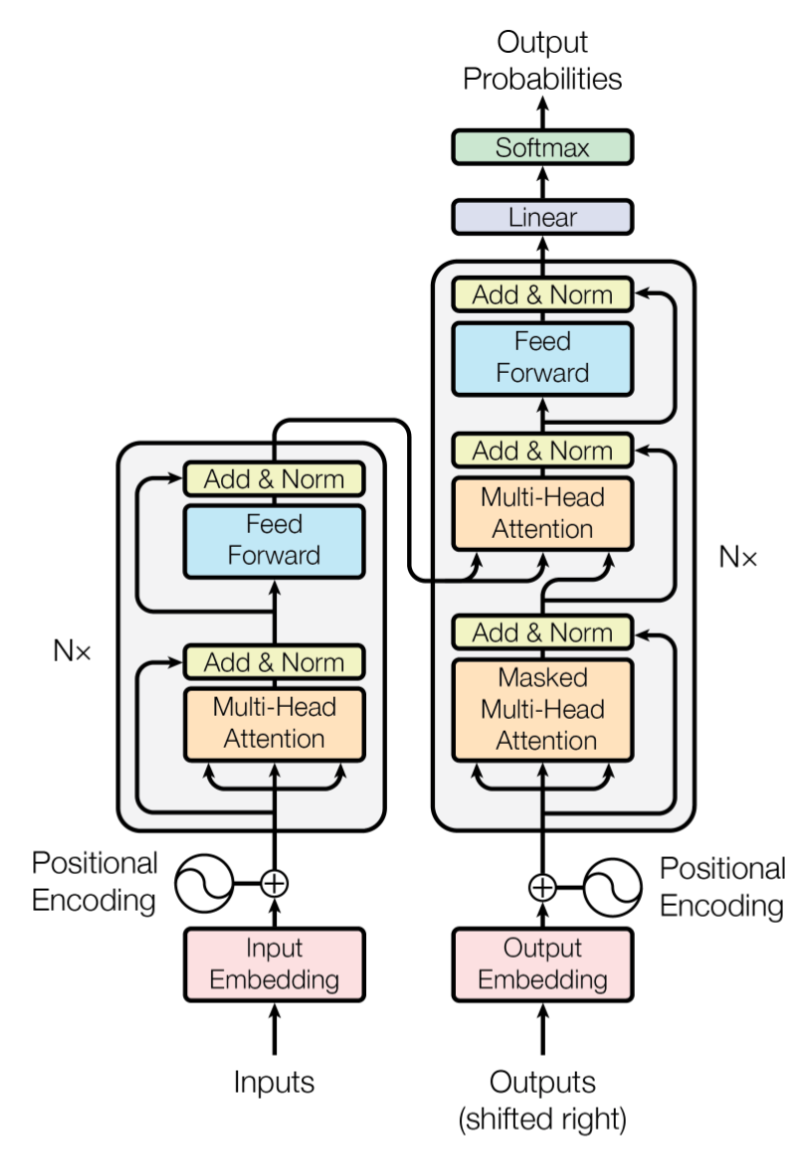
\includegraphics[width=0.45\linewidth]{Images/Transformer_architecture3.png}
    \caption{Transformer Architecture from\cite{vaswani2017attention}}
    \label{fig:Tranformer}
\end{figure}
\subsection{Main Innovations in Transformer Architecture}  
\begin{itemize}
    \item \textbf{Embeddings}: Learned embeddings convert input and output tokens to vectors of dimension $d$ depending on the dimension of the model. Tokens are discrete symbols of words or subwords.
    
    \item \textbf{Positional Coding}:  
    Transformers do not need recurrence nor convolution, instead some information about relative or absolute position of the tokens is injected in the sequences. This is the positional encodings added to the input embeddings. \cite{vaswani2017attention}.  
    \item  \textbf{Scaled Dot-Product Attention}\ref{eq:Attention}: Is an attention function\ref{eq:Attention} that maps a query and a set of key-value pairs to an output.
    \begin{equation}
        \label{eq:Attention}
        \text{Attention}(Q,K,V) = softmax(\frac{QK^T}{\sqrt{d_k}})V 
    \end{equation} 
    \begin{itemize}
        \item Q is a set of keys packed together into a matrix.
        \item K and V are also matrices packed together of keys and values, respectively
    \end{itemize}
    \item \textbf{Multi-Head Attention}:  Queries, keys and values are linearly projected $h$ different times with different learned linear projections\ref{eq:MultiHead}. The Multi-head attention allows the model to jointly attend to information from different representation subspaces at different positions. \textbf{Masked Multi-Head Attention} masks future positions in the sequence during the decoding process\cite{vaswani2017attention}.
    \begin{equation}
        \label{eq:MultiHead}
        \text{MultiHead}(Q,K,V) = \text{Concat}(head_1, ..., head_h)W^O  
    \end{equation}
    \begin{itemize}
        \item $head_i = \text{Attention}(QW_i^Q, KW_i^K,VW_i^V)$
    \end{itemize}
    \item \textbf{Feed-Forward}:  A Position-Wise Feed-Forward Network (FFN)\ref{eq:FNN} is a fully connected neural network designed to independently process each position in the sequence.  While FNN \ref{eq:FNN} operates identically at all positions, the parameters vary between layers. The dimension of the inner-layer has a larger dimension than the model's dimension to increase its capacity to learn complex transformation\cite{vaswani2017attention}.
    \begin{equation}
        \label{eq:FNN}
        \text{FNN}(x) = \max(0,xW_1+b_1)W_2+b_2
    \end{equation}
\end{itemize}




\subsection{Performance and Impact}  
The Transformer architecture achieved top results in machine translation tasks, such as on the WMT 2014 English-German and English-French datasets, with significantly shorter training times compared to previous models. For example, the model achieved a BLEU score of 28.4 on English-to-German translation, outperforming previous architectures by more than 2 BLEU points \cite{vaswani2017attention}.  
The Transformer architecture has had a transformative impact on \ac{NLP} . It serves as the basis for \ac{LLM} models such as BERT, GPT and others, which are based on the core principles of self-attention and scalability.


\section{Vector store}
A vector store (sometimes referred to as a vector database or embedding store) is a specialized system designed to store and query high-dimensional vectors efficiently. Such systems are commonly used during inference to optimize tasks involving vector embeddings (e.g., text search, similarity search, and image similarity). In modern machine learning models—particularly those in \ac{NLP} or computer vision—inputs such as text or images are transformed into high-dimensional embeddings that capture semantic information.

By utilizing a vector store to maintain these embeddings, it becomes possible to query or index them efficiently through specialized algorithms such as \ac{ANNOY}, \ac{HSNW}, \ac{FAISS}, or \ac{IVF}. These algorithms help narrow down the set of candidate vectors quickly, avoiding the need to scan the entire database. Common distance or similarity metrics include:
\begin{itemize}
    \item Cosine similarity: measures the cosine of the angle between two vectors, useful when the orientation of the vector is more significant than its magnitude. 
    \item Euclidean distance: measures the straight-line distance between two vectors in space. Useful when spatial proximity correlates with data similarity.
    \item Dot Product: Accesses the magnitude of the projection of one vector onto another, measuring their similarity in terms of both direction and length. Used to approximate inner products between compressed vectors, enabling efficient similarity computations in large datasets. This method is particularly effective in large-scale information retrieval systems. \ref{eq:dot_sim}
\end{itemize}

Vector stores have gained increasing prominence due to their effectiveness in handling high-dimensional data more efficiently than traditional or NoSQL databases. They also integrate seamlessly with \ac{LLM}, making them indispensable in modern AI pipelines.


\section{\acl{RAG}}
Improve this explanation, explain the 3 steps of RAG more clearly
\ac{RAG} is a system that used for tackling knowledge-intensive \ac{NLP} tasks by combining parametric knowledge, knowledge from the \ac{LLM}s parameters,  with non-parametric memory sources, information from another source. In other words enhancing a pre-trained \ac{LLM} with a retrieval component that can access external documents during generation, rather than relying solely on the model's internal parameters.
\subsection{Parametric and Non-Parametric Knowledge}
Traditional pre-trained \ac{LLM} store their knowledge implicitly in their parameters, this is the parametric knowledge. While they can encode a vast amount of information, their stored knowledge is static and can be out-of-date. \ac{RAG} augments these models with a retrieval component that provides up-to-date and explicit external knowledge, non-parametric knowledge, thereby reducing reliance on parametric knowledge in the model.

\subsection{Sparse Retrieval Methods}
Are methods that work with sparse representations of text. this representations are known as keywords, terms.
The component that specializes in how the information is retrieved from the database to the model. Here we will revise a few retrieval methods that have been developed and used.
\subsubsection{TF-IDF (Term Frequency-Inverse Document Frequency)}
TF-IDF is a foundational term-weighting and ranking scheme in information retrieval systems \cite{tf-idf}. Its primary purpose is to measure how important a term is to a particular document within a large collection of documents. While frequency counts can highlight terms that often appear, they do not account for how common or rare those terms are across the entire dataset. TF-IDF addresses this by diminishing the weight of terms that occur frequently across many documents (common words)  and increasing the weight of terms that appear in fewer documents (more distinctive terms).
The \ac{TF} measures how often a term \textit{t} appears in a single document \textit{d}. 
\begin{equation}
    \label{eq:tf} 
    \text{TF}(t,d)=f_{t,d}
\end{equation}
For longer documents a normalization is used a such:
\begin{equation}
    \label{eq:tf(t,d)}
    \text{TF}(t,d) = \frac{f_{t,d}}{\sum_{t'}f_{t',d}}
\end{equation}
The inverse document frequency (IDF) measures how common a term is across the entire collection of documents. If a term appears in many documents, it is less useful for distinguishing those documents. A higher IDF means a term appears in fewer documents, indicating its uniqueness. \textit{N} is the total number of documents in the collection, and $n_t$ is the number of documents in which the term appears. \textit{IDF} is defined as:
\begin{equation}
    \label{eq:idftf}
    \text{IDF}(t)=\log\frac{N}{n_t}
\end{equation}
TF-IDF is then the combination of both TF and IDF
\begin{equation}
    \label{eq:tfidf}
    \text{TF-IDF}(t,d) = f_{t,d} \times \log\left(\frac{N}{n_t}\right)
\end{equation}
The uniqueness of the TF-IDF approach in retrieval is how it combines a local component (frequency in the current document) and a global component (frequency across the entire collection). TF-IDF has the advantage of being straightforward, interpretable, and computationally efficient.

\subsubsection{BM25 (Okapi BM25)}
The okapi system first introduced in\cite{Bm25foundation} which then culminated to BM25. The BM25(short for "Best Match 25") is a probabilistic information retrieval model. This information retrieval model improves upon TF-IDF by using a probabilistic basis rather than a purely heuristic bases, and by introducing parameters to control term frequency by saturation, and document length normalization.
The BM25 formulas is similar to the TF-IDF as it uses a more sophisticated formulation of the IDF component found in TF-IDF this one is more stable and empirically effective. The IDF component per term \textit{t} is computed as:
\begin{equation}
    \label{eq:idfbm25}
    \text{IDF}(t) = \log \frac{N-n_t+0.5}{n_t+0.5}
\end{equation}
where N is the total number of documents in the collection and $n_t$ is the number of documents containing term \textit{t}.

BM25 formula to score a document from a query( a number of terms) looks like \cite{bm25}:
\begin{equation}
    \label{eq:bm25}
    \textit{BM25}(d,q) = \sum_{t \in q} IDF(t) \cdot \frac{(k_1+1)\cdot f_{t,d}}{f_{t,d}+k_1(1-b+b \cdot \frac{|d|}{avgdl})}
\end{equation}
where:
\begin{itemize}
\item $d$ is a given document.
\item $q$ a user's query, consisting of t terms.
\item $|d|$ is the length of a document in terms of the number of tokens.
\item $dl$ is document length $:=\sum_{i \in V}{tf}_i$
\item $avgdl$ is average document length across the entire collection
\item $k_1$ and $b$ are tuning parameters:
\begin{itemize}
    \item $k_1$ controls  the saturation of \ac{TF}, by preventing over-emphasis on very frequent terms.
    \item $b$ controls the amount $dl$ is normalized. If $b = 1$, the normalization is directly proportional to how much longer( or shorter) the document ($|d|$) is compared to average document length ($avgdl$). if $b=0$, no document length ($dl$) is applied.
\end{itemize}
\end{itemize}

\subsection{Vector-based Retrieval Methods}


Retrieval of a relevant document from a large collection, based on a user query, was traditionally implemented using TF-IDF or BM25 \cite{bm25}. These are sparse vector space models that match keywords efficiently via an inverted index. Under such methods, both queries and documents are represented as high-dimensional, sparse vectors with term-based weighting. While these models are often effective for keyword-based matches, they struggle when queries and relevant documents use synonyms or paraphrases that do not share surface-level terms.

Recent advancements in \ac{LLM}, particularly transformer-based models like BERT \cite{bertpretrainingdeepbidirectional}, have led to dense retrieval systems. In dense retrieval, queries and documents are represented as low-dimensional vectors that better capture semantic similarity. However, dense methods often require large training datasets (i.e., labeled question–passage pairs) to surpass classical methods such as TF-IDF/BM25. Modern pre-trained language models help mitigate this requirement by providing robust initial embeddings that can be fine-tuned on relatively smaller sets of question–context examples. This opens the door for dense retrieval methods to outperform traditional sparse approaches in many open-domain QA tasks.
\subsubsection{Dense Passage Retrieval (DPR)}
\label{par:dpr}
Dense Passage Retrieval (DPR), introduced by Karpukhin et al.~\cite{densepassageretrievalopendomainkarpukhin2020}, is a \textit{dense retrieval} method designed specifically for \textit{open-domain question answering}. Unlike conventional approaches that rely on \textit{purely lexical} matches (e.g., TF-IDF and BM25), DPR employs BERT-based encoders to map questions and passages into a shared, dense embedding space, enabling \textit{semantic} rather than strictly \textit{keyword-based} retrieval. By leveraging modern \ac{LLM} such as BERT~\cite{bertpretrainingdeepbidirectional} and LLaMA, which come with strong pre-trained representations, DPR can be fine-tuned with comparatively fewer labeled samples. This allows the system to capture semantic relationships between questions and passages, thereby mitigating the shortcomings of traditional methods that rely solely on term overlap.

The DPR architecture is based on a dual-encoder architecture~\cite{dualencoderarchitecture}. Specifically, in Karpukhin et al.'s formulation~\cite{densepassageretrievalopendomainkarpukhin2020}, both encoders are initialized from the same pre-trained BERT model but are then fine-tuned separately for their respective tasks. A Question Encoder \(E_Q\) takes a question as input and produces a single vector embedding \(q_i\), while a Passage Encoder \(E_P\) processes a passage to produce a single vector embedding \(p_j\). Once encoded, each question and passage becomes a fixed-dimensional vector (e.g., 768 dimensions). To measure the similarity between a question \((q)\) and a passage \((p)\), the dot product of their embeddings is computed:
\begin{equation}
    \label{eq:dot_sim}
    \text{similarity}(q, p) = E_Q(q)^T \, E_P(p).
\end{equation}

For very large document collections (e.g., a full Wikipedia dump), a dense vector index like \ac{FAISS} \cite{DOUZE2024FAISS} is typically used to support efficient similarity searches. \ac{FAISS} is a specialized library designed for rapid similarity search and clustering of dense vectors, enabling the system to scale to billions of embeddings. Concretely, DPR encodes all passages offline with \(E_P\), storing the resulting passage embeddings \((p_j)\) in the \ac{FAISS} index. This offline procedure ensures that the more computationally intensive step—embedding the entire corpus—happens only when the vector database needs to be updated.

%\subsection{Rag Variants}

%\=printf("\ac{%s}", toupper(submatch(1)))rag} is a novel approach to \ac{nlp} that aims to improve the performance of \acpl{llm} on knowledge-intensive tasks. \ac{rag} overcomes limitations of existing \acpl{llm} by combining a pre-trained sequence-to-sequence (seq2seq)  model (parametric memory) with a dense vector index to a vector database acessed via a neural retriever (non-parametric memory). Parametric memory, comes from the generator component \ac{llm} itself. the non-parametric memory is part of the retrieval component,  based on a bi-encoder architecture. A document encoder produces a dense representaion of a document, and a query encoder produces a representation of the input query. The retriever is initialized using a pre-trained bi-encoder that has been trained to retrieve documents containing answers to questions. There reason why it is important to differentiate parametric memory with non-parametric memory is that they have some key differences. Non-parametric memory for can be easily updated by replacing the document index, is also more interpretable because it consists of raw text that is human readable, 

%What is \acentrylong{rag} and why is it so important in organizations.\=printf("\ac{%s}", toupper(submatch(1)))llm} have shown that they are able to store factual knowledge in their parameters. And by themselves can give information. The problem is that to add information to it, the model must be trained again. Also the model can give you information, but will not provide the source of information. So the information cannot be verified, and so it cannot be used in a corporate environment, as \ac{llm} can also hallucinate knowledge.

%\section{Access Control Lists}

% #############################################################################
